In this chapter we present  \namens,  an open source framework for Systematic Comparative Research on RSP Engine.
It consists in four baselines and two main components: the Test Stand and the Analyser. Firstly, Section \ref{sec:teststand} introduces the Test Stand, which satisfies requirements from R.1 to R.8 and from R.10 to R.12, by executing experiments on an RSP Engine. Section \ref{sec:baselines} describes the Baselines, four RSP Engines that are included in \name as naive terms of comparison, since they fulfil requirements R.13 and R.14. Finally, Section \ref{sec:analyser} presents the Analyser, which addresses requirements R.9 and R.10  allowing the user to visualise, investigate and compare experiment results. %Soundness and completes of the query answering process are assessed post-hoc by comparing the results of an RSP engine with a term of comparison whose results are correct (see Section 5).

\section{Test Stand}\label{sec:teststand}

Aerospace engineering defines an engine test stand as a facility used to develop, study and characterise engines. It allows to test operating regimes and offers measurement of several variables associated with engine process. A test stand may uses actuators for attaining a specific engine state, which is a unique combination of the engine properties. The information collected through the sensors depends on the engine manufacturer, which usually provides his own stand or the facilities to test the engine with commercial solutions. The test stand executes black box testing over engines, because its users can not rely to known engine internal mechanisms.

The definition above still holds its relevance in the SR context, with the difference that engines subject of the testing, RSP Engines, are IO-Systems. An RSP Engine consumes an RDF Stream and  produces a new one, by applying queries under some entailment regime and w.r.t. an ontology which does not change over time. Describing an RSP Engine means understanding the relation between input stream, the queries registered to it and what we call \textit{operational semantics}, which requires to know the RSP Engine internal processes. Indeed, black box testing is the only possibility to analyse such system with a test stand. Even having access to the entire RSP Engine code, may results hard to characterise all the RSP Engine properties a priori. 

Figure \ref{fig:architecture} shows \name \textsc{Test Stand} design. It contains the block schema of the modules that composes the \textsc{Test Stand} pipeline. Moreover, we enumerates in the Figure the events that pass trough the the \textsc{Test Stand} while it is executing and experiment. In the following subsection we describe each elements that Figure \ref{fig:architecture} summarises. In Subsection \ref{sec:modules} we describe the \textsc{Test Stand} pipeline and each module that composes it, in Subsection \ref{sec:test-stand-data-model} we detail the Data Model exploited to represent experiments, events, query results and measurements. Finally, in Subsection \ref{sec:test-stand-workflow} we describe the \textsc{Test Stand} workflow, how it executes experiments to stress the RSP Engine we want to test.

\begin{figure}[tbh]
\centering
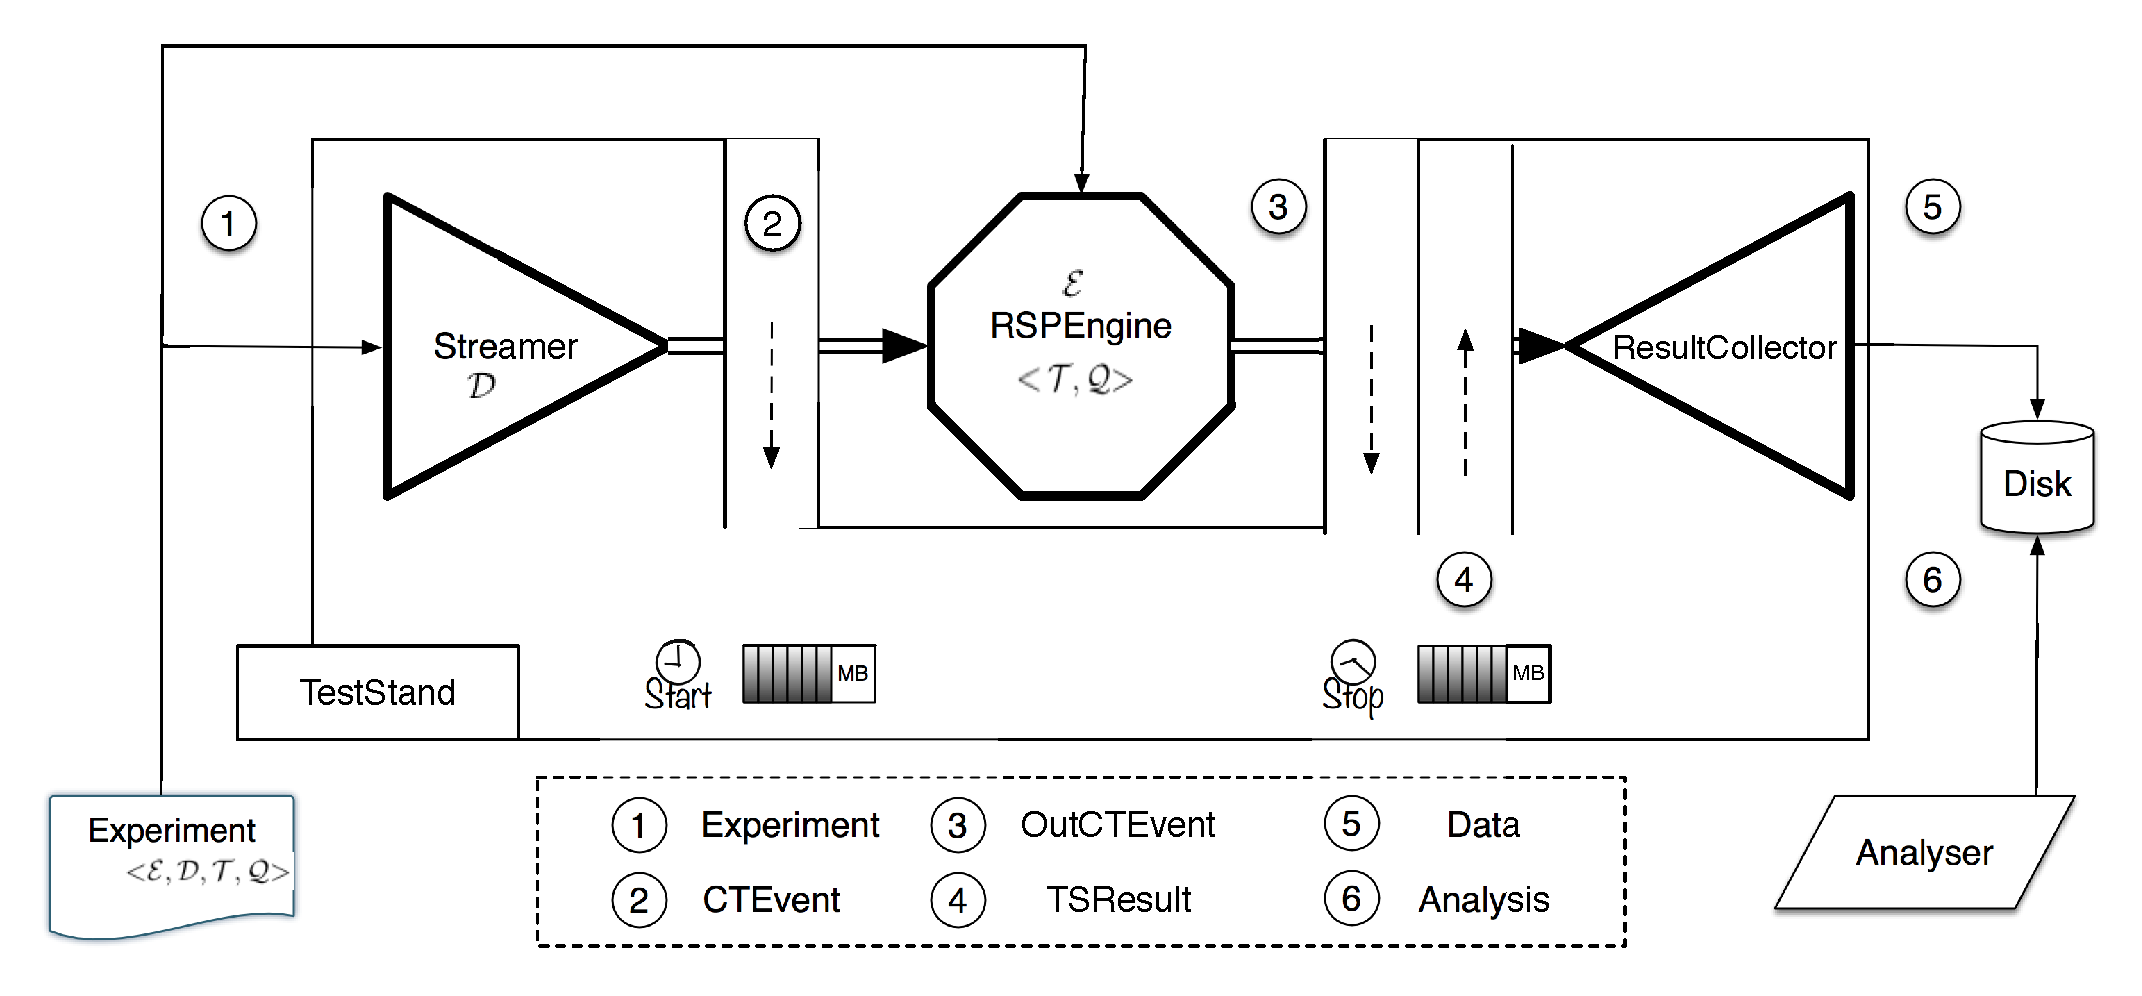
\includegraphics[scale=0.37]{images/schema2}
\caption{\name modules and workflow} 
\label{fig:architecture}
\end{figure}


\subsection{Modules}\label{sec:modules}

\noindent An aerospace test stand exploits different modules to simulate the operating regime for the engine in use ( i.e a module for fuel distribution, one for the engine mechanic support or to enable users interaction during the execution ). Modularity allows to extend the test stand and specify testing procedure. 

We design \name \textsc{Test Stand} as modular system for the same reasons, guaranteeing modularity [R.10]. Thus, it consists into the following three stand-alone modules:
\begin{itemize}
\item the \textsc{Streamer}, a source for the input RDF Stream
\item the RSP Engine we want to test;
\item the \textsc{Result Collector}, a data acquisition system for both the query results and the gathered measurements.
\end{itemize}

\noindent The architecture of \name \textsc{Test Stand} is represented in Figure \ref{fig:architecture}. The \textsc{Test Stand} modules  are arranged into a pipeline and communicates exchanging events [R.11]. Their interfaces allow each of them to be replaceable with an other ones with a different behaviour, but which complies with the interfaces specifications.

The execution starts with the \textsc{Streamer}, which hides the data generation logic in order to obtain data independence [R.1]. It pushes an RDF Stream directly to the mounted RSP Engine. It is up to the \textsc{Streamer} to respect [R.5] and not to influence the memory footprint with heavy data loading tasks. 

An interface adapts the event flow to the RSP Engine in use, fulfilling [R.2] (Engine Independence) and hiding the query registration process [R.3] (Query independence), which happens at engine level and is up to the RSP Engine provider.

The \textsc{Result Collector} is at the tail of the pipeline. It is part of the \textsc{Test Stand} because the performance measurements are processed and gathered during the execution, together with the queries results data. The \textsc{Result Collector} is responsible to save all this data at the end of each cycle, without influencing the system. The evaluation usually happens a-posteriori trough the Analyser (Section \ref{sec:analyser}). However, real time analysis of the performance measurements are possible, but they may violate some requirements like [R.4] and [R.5]. 

Last but not least, the Test Stand has an external structure that sustains other modules and can be considered as a module itself. It allows the user to control the process through accessible APIs. It gathers the data sampled by the sensors during the execution and adds them to the query results. The \textit{Test Stand} External Structure allows the user (the RSP Engine developer) to develop a specific testing procedure for a given engine. The measure set extensions are possible by adding user defined metrics, according to requirements [R.7] and [R.10]. Finally, it controls the process ensuring that the \textsc{Test Stand} does not run when the RSP Engine run as required by [R.4].

\subsection{Experiment \& Data Model}\label{sec:test-stand-data-model}

\noindent The Test Stand accepts as input an \textsc{Experiment} in the form of a tuple \\ $<\mathcal{E},\mathcal{D},\mathcal{T},\mathcal{Q},>$ where:
\begin{itemize}
\item $\mathcal{E}$ is the RSP Engine subject of the evaluation (satisfying requirement [R.3]); 
\item $\mathcal{D}$ is the input dataset [R.1]; 
\item $\mathcal{T}$ is the ontology [R.1]; 
\item $\mathcal{Q}$ is the query to be continuously answered by $\mathcal{E}$ [R.2]. 
\end{itemize}

From an experimental point of view, which metrics we sample during the execution have a different influence on the measurements. For example, asking to the system for the memory usage may influence the latency calculus or saving on disk the query results may influence the memory footprint. Thus, we define there main kinds of experiment, distinguishing on the data we want to sample and save. Notice that which experiment kind choose depends on the goal and the error tolerance of the research.

\begin{itemize}
\item Latency Experiment, where only the latency is calculated and no query result is saved on file
\item Memory Experiment, where only the memory is gathered and no query result is saved on file
\item Query Experiment, where query results are saved on file.
\item Any combination of the previous experiment types.
\end{itemize}


\noindent In order to describe the Data Model exploited by the \textsc{Test Stand}, we draw the Entity-Relation diagram in figure \ref{fig:er}. The diagram does not include entity attributes to simplify the interpretation, but they are reported in the following Logic Schema:
\begin{figure}[tbh]
  \centering
	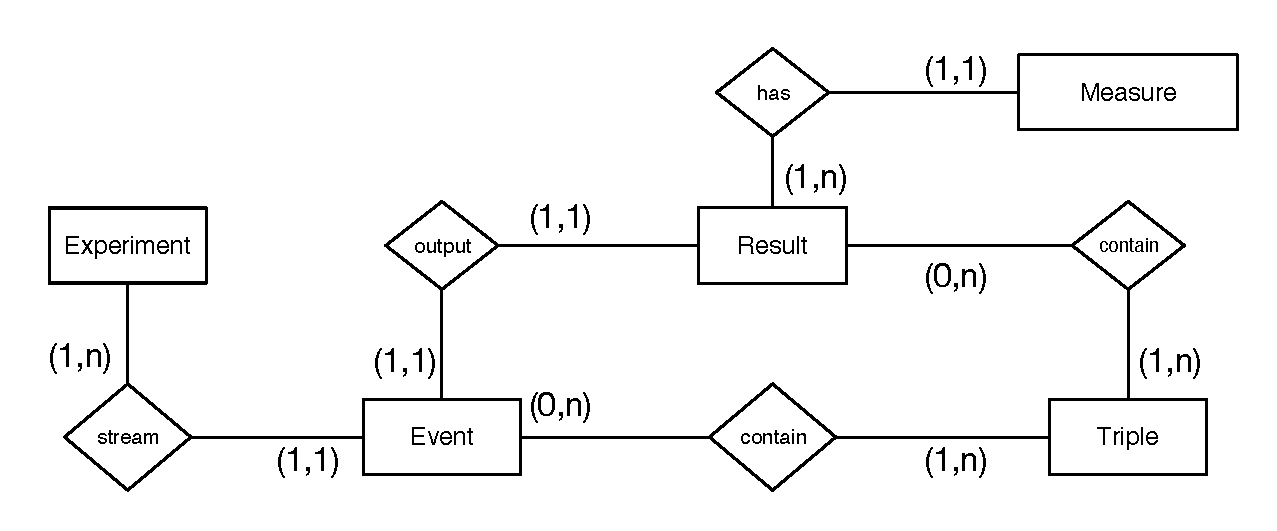
\includegraphics[width=\linewidth]{images/er-db}
	\caption{ER-Diagram For Experiment Output} 
  	\label{fig:er}
\end{figure}\\
\noindent\textsc{Experiment}(\underline{ID}, Timestamp Start, Timestamp End, Engine, Ontology, Query, Dataset, Description)\\
\textsc{Event}(\underline{ID, Experiment ID}, Timestamp)\\
\textsc{Result}(\underline{Result ID, Experiment ID}, Event ID)\\
\textsc{Measure}(\underline{ID}, Value)\\
\textsc{Measurement Set}(\underline{Measure ID, Result ID, Experiment ID})\\
\textsc{Triple}(\underline{S,P,O})\\
\textsc{Output Triple}(\underline{Result ID, Experiment ID, S, P, O})\\
\textsc{Input Triple}(\underline{Event ID, Experiment ID, S, P, O})\\

The \textsc{Experiment} entity contains the metadata of the tuple $<\mathcal{E},\mathcal{D},\mathcal{T},\mathcal{Q},>$, which semantic is explained above. "Timestamp Start" and "Timestamp End" are relevant metrics for further analysis and system control. 

The \textsc{Event} is unique inside an \textsc{Experiment}, it is possible to send two events with the same timestamp and identical tripleset. The Timestamp field allows to order events after the execution

The \textsc{Result} is associated with one and only one \textsc{Event}. It contains the results to the engine queries w.r.t the active window and the set of the measure gathered during the execution. 

The \textsc{Measurement Set} table represents the many-to-many relation between the \textsc{Result} and a number of measure that may variate  to fulfil requirement [R.7] (extendible measurement set). 

We include the concept of the \textsc{Triple} in order to model the content of \textsc{Event} and \textsc{Result}. \textsc{Input Triple} and \textsc{Output Triple} are the tables which represent two many-to-many relations, respectively between \textsc{Triple} and \textsc{Event} and \textsc{Triple}  and \textsc{Result}

\subsection{Test Stand Workflow}\label{sec:test-stand-workflow}

\noindent The \textsc{Test Stand} orchestrates the communication between the upstanding models, forcing the \textsc{Streamer} to push events to the RSP Engine and the \textsc{Result Collector} to listen the output and collect the results. To explain the \textsc{Test Stand} workflow we split the process at the points when the modules exchange events. Indeed, each message represents a different logic step in the experiment execution cycle.

Six different steps are identified by six events exchanged by \textsc{Test Stand}, \textsc{Streamer} and RSP Engine. The \textsc{Result Collector} only receives events, terminating each cycle.

In step (1) the \textsc{Test Stand} takes the experiment and starts the execution. It executes the experiment $<\mathcal{E},\mathcal{D},\mathcal{T},\mathcal{Q},>$ stressing $\mathcal{E}$ for a certain period of time looping through the steps from (2) to (5) illustrated in Figure \ref{fig:architecture}.                                                                                                                                                                                                                                                                                                                                                                                                                                                                                                                                                                                                                                                                                                                                                                                                                                                                                                                                                                                                                                                                                                                                                                                                                                                                                                                                                                                                                                                                                                                                                                                                                                                                                                                                                                                                                                                                                                                                                                                                                                                                                                                                                                                                                                                                                                                                                                                                                                                                                                                                                                                                                                                                                                                                                                                                                                                                                                                                                                                                                                                                                                                                                                                                                                                                                                                                                                                                                                                                                                                                                                                                                                                                                                                                                                                                                                                                                                                                                                                                                                                                                                                                                                                                                                                                                                                                                                                                      

In step (2), the \textsc{Streamer} pushes to $\mathcal{E}$ an event \textsc{CTEvent}. This event is a portion of an RDF Stream picked from the data $\mathcal{D}$ and it consists of a set of RDF triples with the same timestamp. In order to satisfy [R.12], it sends triple in N-Triple\footnote{\url{http://www.w3.org/2001/sw/RDFCore/ntriples/}}, which is the easiest RDF serialisation to parse.  


In step (3) $\mathcal{E}$ pushes to the \textsc{Result Collector} an event \textsc{OutCTEvent}. It contains the current answer to the query $\mathcal{Q}$ registered in $\mathcal{E}$ given the ontology $\mathcal{T}$. The \textsc{Test Stand} expects $\mathcal{E}$ to output result in N-Triple format. 

Notably, to place any RSP engine on the \textsc{Test Stand} (requirement [R.3]) \name provides a simple software wrapper that, when it receives a \textsc{CTEvent}, adapts it to the RSP engine specific format, pushes it in the RSP engine, and listens to the RSP engine output so to transform such an output in a \textsc{OutCTEvent}.

To measure performances (requirement [R.6]) the \textsc{Test Stand} performs several actions both before step (2) and after step (3) to collect data from the sensors. Previous works about Stream reasoning \cite{DBLP:conf/esws/ScharrenbachUMVB13} shows that the minimal performance measure set includes \textbf{Latency} -- defined as the delay between the injection of an event in the RSP engine and its response to it --, \textbf{Memory Load} -- defined as the difference between total system memory and the free one --, and \textbf{Completeness \& Soundness} of query-answering results. To measure latency, it starts a timer before (2) and stops it after (3). To measure memory load, it asks for the free memory of the system after step (3). Completeness \& Soundness are evaluated with post-processing analysis of the query results data.

In step (4), those observations are added to the outputs of $\mathcal{E}$ as annotations and are pushed to the \textsc{Result Collector}.  We name \textsc{TSResult} the event that contains the sensor data plus the query results produced by the engine.  

The \textsc{Test Stand} works in a single thread mode, blocking the execution of its components when it performs the measurements in (2) and (3) [R.4].  

In step (5) the \textsc{Result Collector} saves \textsc{TSResult} for post process analysis [R.9], executed trough the \textsc{Analyzer}. It does so saving the content of any TSResult  [R.8].

\section{Baselines}\label{sec:baselines}

\noindent In Chapter \ref{chap:problem-settings} we state that a Systematic Comparative Research Approach needs initial terms of comparison to lead the investigation. \name contains a set simple and easy-to-use RSP Engines called "Baselines". As the name lets to guess, these engine fulfil the four characteristics, detailed in Section \ref{sec:requirements}, required by an RSP Engine to be classified as a baseline inside the SR research field. Thus, \name Baselines are \textit{Elementary}, \textit{Relevant}, \textit{Simple} and \textit{Eligible}. developed to fulfil this lack. 

%We exploit them to define some qualitative methods of investigation and to prove the usability of the Test Stand. 
Early works on SR \cite{DBLP:conf/fis/ValleCBBC08,Walavalkar08streamingknowledge} describe the most simple approach to create a stream reasoning system: pipelining a DSMS with a reasoner. The DSMS is responsible to handle the data stream, moving from infinite sequences to finite (and processable) sets of events. The reasoner instead applies SPARQL queries on this set of events, exploiting its reasoning capabilities over a context that can be considered as static, but remains continuous. We focus on RDF Stream Processing, whose foundations, as explained in Section \ref{sec:sfp}, are: 
\begin{enumerate}
\item[1.] RDF streams, detailed in Section \ref{sec:rdfstream}
\item[2.] An extensions of SPARQL to manage continuous data (see Section \ref{sec:continuous-sparql}
\item[3.] reasoning algorithms
\end{enumerate}

\begin{figure}[tbh]
  \centering
	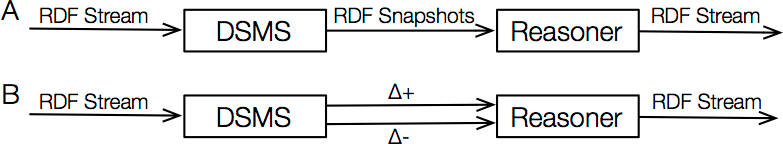
\includegraphics[width=\linewidth]{images/baselines-final}
	\caption{A: the architecture of the Naive baselines. B: the one of  the Incremental ones.} 
  	\label{fig:baselines}
\end{figure}

\noindent RSP Engine are those systems that can apply reasoning techniques upon rapidly changing information encoded in RDF (RDF Stream) and allow to continuous querying on the data stream (Section \ref{sec:rspengine}). It possible to develop RSP Engine following the approach described above, which actually requires to develop the integration of two existing technologies, DSMS and reasoner, and to define how they can communicate. Following we describe how this design model fulfil the requirements we posed in Section \ref{sec:requirements}.

Baselines \textit{Elementarity} can be granted by choosing a DSMS which is a reliable solution in the Information Flow Processing context and the a general purpose rule engine which is comparable with mature solutions. \textit{Elementarity} is reached when the couple elements are simple and valid terms of comparison w.r.t the state of the art.

Baselines \textit{Relevance} requires to cover all the most important theoretical variants that the "pipeline approach" conveys. In terms of reasoning we can choose between two possible approaches and with reference to the data stream processing the choices are again two. Four baseline implementations cover these two main design decisions about the RDF Stream Model and the Reasoning procedures. 

The RDF Stream model describes how the input RDF Stream is processed, different systems accept data in different models, which depends on how RDF Stream is considered in terms of events contemporaneity. The two most relevant ones are:

\begin{itemize}	
\item Triple-based model, where the events pushed in the DSMS are timestamped triples. The timestamps are non decreasing, different triples could have the same timestamp to denote that they are contemporary.
\item RDF Graphs-based: the event pushed in the DSMS are timestamped RDF graph. The timestamps are increasing and the graph is used as a form of punctuation \cite{Tatbul2003b} to separate consequent portions of the RDF stream.
\end{itemize}

The Reasoning Architecture, the techniques to make inference, depends on the way data flow from the DSMS to the reasoner. Two reasoning solutions exist for the two triples data flow:

\begin{itemize}
\item Naive solution: (Figure \ref{fig:baselines}-A) the DSMS produces an RDF Snapshot of the current windows. It sends the entire content of the window to the reasoner, which materialises all the implied triples at each cycle. This is the approach implemented in the C-SPARQL Engine \cite{DBLP:journals/sigmod/BarbieriBCVG10} and in Sparkwave \cite{DBLP:conf/debs/KomazecCF12}.
\item Incremental solution (Figure \ref{fig:baselines}-B) the DSMS outputs the IRStream, the differences between the current window and the previous one. The $\Delta^{+}$ snapshot contains the triples that have just entered in the window, while the $\Delta^{-}$ snapshot contains the triples that have just exited from the window. The reasoner, using $\Delta^{+}$ and $\Delta^{-}$, incrementally maintains the materialisation over time. This approach is taken as term of comparison in \cite{DellAglio2014} and it is inspired from \cite{DBLP:conf/cikm/RenP11}.
\end{itemize}

Baseline \textsc{Eligibility} requires to check out all the performance measurements involved by the RSP Engine in use. We already stated that the choice of the DSMS and the reasoner may affect baseline \textsc{Elementarily}, but they also influence the performance of the engine. In order to be Eligible the Baselines must be comparable with mature solutions in terms of degree of magnitude. As reported in Section \ref{sec:teststand}, we take as initial measure set: Latency, Memory and of the query results Completeness and Soundness. Latency and Memory are the metrics upon which the comparison can be built. Further consideration can be done for Completeness and Soundness w.r.t recent work on correctness \cite{DBLP:conf/semweb/DellAglioCBCV13}  \cite{DBLP:conf/semweb/DellAglioCBCV13} explains the importance of external control on time to assure that the RSP Engine always outputs the correct answers (even when overloaded). The proposed Baselines should take advantage of the ability of some DSMS to be temporally controlled by an external agent by sending time-keeping events to synchronise the internal time flow. In this wat is possibile to ensure Completeness and Soundness even in case of high stress condition for the Baselines. %One time-keeping event is sent before injecting the triples in a \textsc{TCEvent} and another one after all triples in \textsc{TCEvent}  were sent. In this way all the triples in the TCEvent are consider contemporary by the 

Finally, baselines \textsc{Simplicity} comes from those parameters that directly influence the RSP Engine: the query $\mathcal{Q},$ and the entailment regime. $\mathcal{Q}$ should be eligible in terms of reasoning which means having an high materialisation effort of the implicit information entailed by the content of the window, given the ontology chosen by the user. The entailment regime should be a fragment of a language, maybe RDF-S, which reduces complexity but preserves the normative semantics and the core functionalities. Moreover, what we state above about externally time control clarifies the system workflow providing \textsc{Simplicity} too.

\section{Analyser}\label{sec:analyser}

The \textsc{Analyser} consists, from an engineering point of view, in one or more automated procedures that process the experiment results transforming raw data into an human-readable form. Actually, not all the analysing procedures can be completely automated and data analysis can not be always generalised. For this reason we decide to design the \textsc{Analyser} from a research point of view. It can bee seen as set of methods for data processing and analysing, which allow to refute or confirm hypothesis and to improve existing models trough empirical findings.

In this Section we focus on the definition of the methods that compose the analysis, while in Section \ref{sec:analyser-impl} we detail much more which tools sustain the investigation at different levels, allowing data visualisation and deeper statistical investigations.

\begin{figure}[tbh]
  \centering
	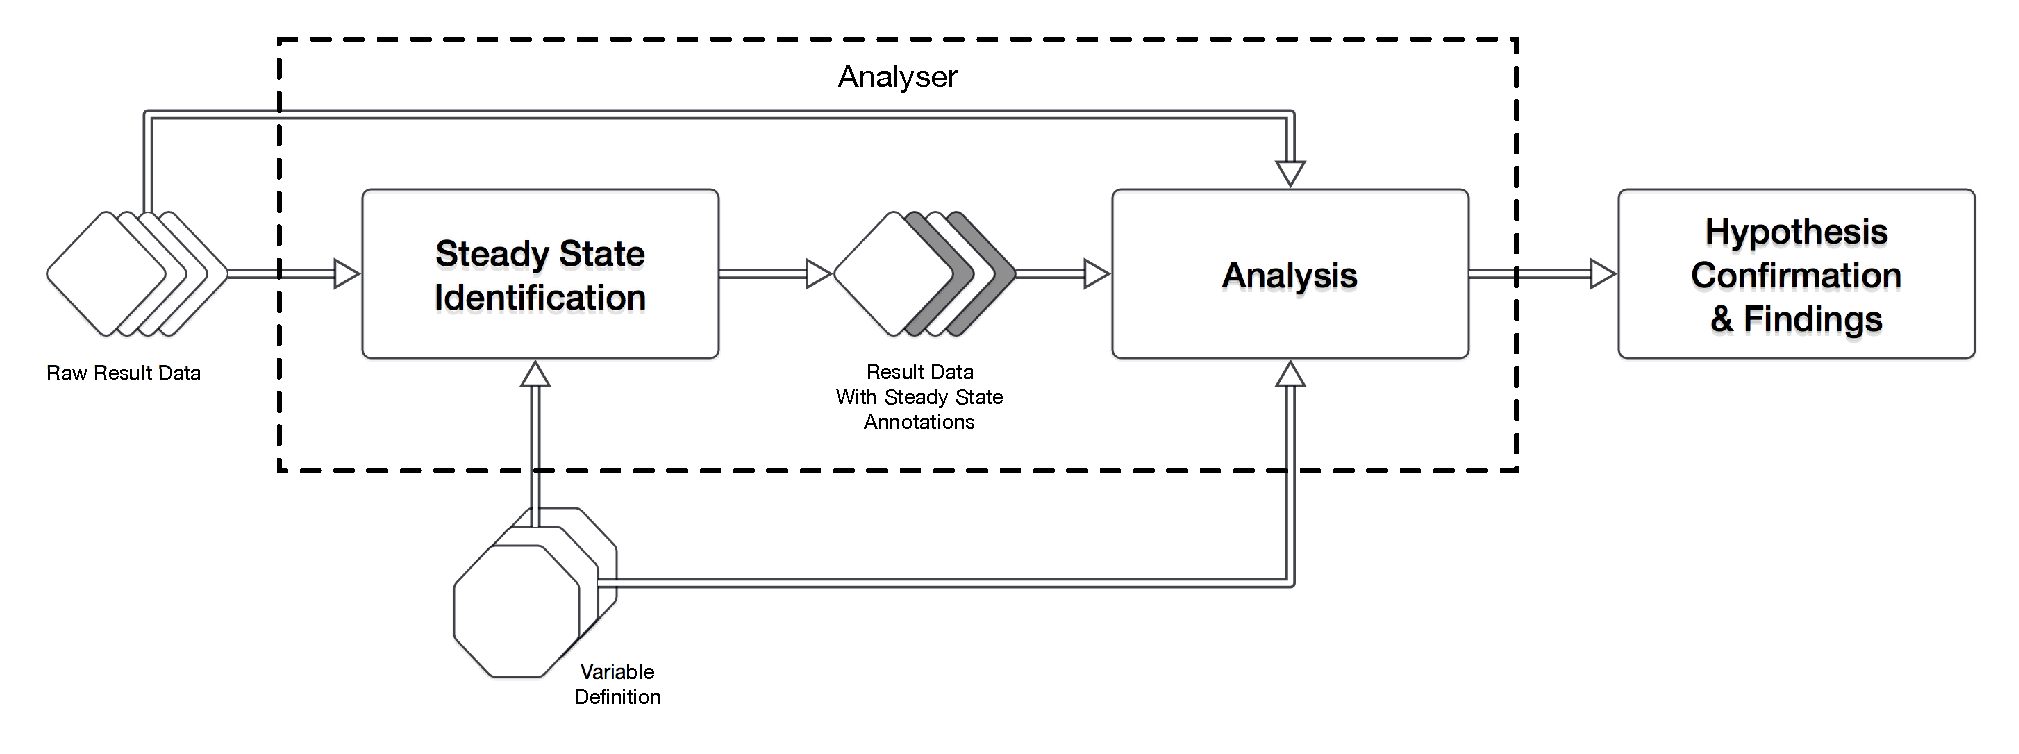
\includegraphics[width=\linewidth]{images/analyser-block-schema}
	\caption{\textsc{Analyser} Block Schema} 
  	\label{fig:analyser-block-schema}
\end{figure}

Figure \ref{fig:analyser-block-schema} shows the different phases of the data processing. The methods that compose the \textsc{Analyser} can be divided into three main block, each one with different supporting tools and different goals.

\textsc{Analyser} takes as input the raw data produced by the \textsc{Test Stand} by executing the experiment, and the variables on which the analysis will be based on. The \textsc{Test Stand} outputs raw data are in times series format and which data it outputs depend on the users needs. The \textsc{Test Stand} measurement set may variate according to the requirement [R.7]. To this extent the \textsc{Analyser} should be extendible too, and the variables of the analysis must be seen as an input provided by \name user.

To properly compare results between $n$ different RSP Engines data must be standardized. In the \textit{Steady State Identification} Block data are processed according to the variables, identifying which variable has reached a Steady State condition.

The last step in the high level Analyser Block Schema consists in the formalisation of theoretical results. The aim of this step is obviously confirm or refute hypothesis formulated at experiment design level. However, \name has the aim of sustaining the empirical research over RSP Engine which allow a new kind of observation that may improve existing theoretical models of the Stream Reasoning area.

In the next subsection we provided further details on the \textit{Steady State Identification} Block, Subsection \ref{sec:analyser-ss-block}, and about the \textit{Analysis} Block, Subsection \ref{sec:analyser-analysis-block}. The Theoretical Result Block it is not described because it depends on \name user and can not be formalised yet.

\subsection{Steady State Identification Block}\label{sec:analyser-ss-block}

\begin{figure}[tbh]
  \centering
	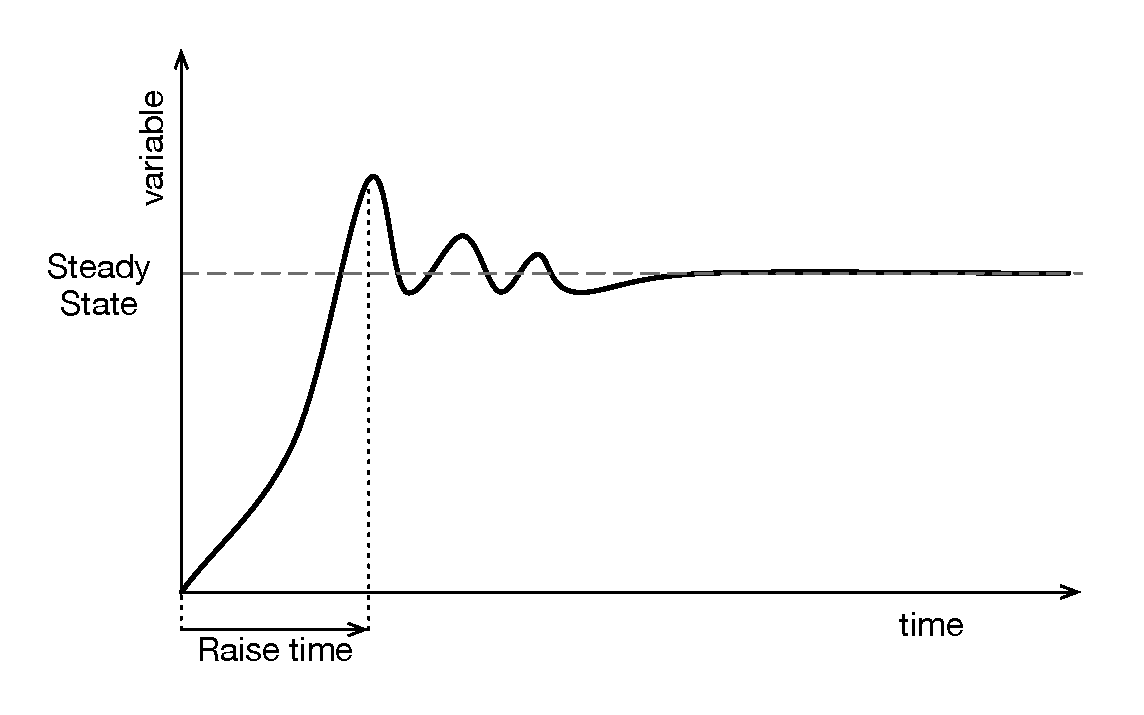
\includegraphics[width=0.5\linewidth]{images/steady-state}
	\caption{Time Series temporal domain} 	
  	\label{fig:steady-state}
\end{figure}

The \textit{Steady State Identification} (SSI) Block is first element in Figure \ref{fig:analyser-block-schema}. In general it applies a pre-analysis of the raw data. It outputs if a given variable of the tested RSP Engine has not reached the Steady State condition , which is the moment when a dynamic system reaches the equilibrium for a certain variable. The SSI is a common passage in almost any research on dynamic system, because those systems usually have an initial transitory phase which inhibits generalisation and comparisons. Figure \ref{fig:steady-state} shows the typical behaviour in the time domain for a certain variable and also evidences the point when the series reaches the Steady State condition. The \textit{Steady State Identification} Block allows to understand the degree of reliability of the data, how we can assume a certain observation is confirmed and generalizable. % 


\subsection{Analysis Block}\label{sec:analyser-analysis-block}

Once the Steady State is identified, it is possible to proceed with the central data analysis, which is summarised in Figure \ref{fig:analyser-block-schema} by the \textit{Analysis} Block. This Block exploits the \textit{Steady State Identification} output to study the transitory phase, which is a crucial part of the dynamic system comprehension and thus of the Hypothesis confirmation.

The investigation can be decomposed in four levels within the \textit{Analysis} Block, with increasing details degree and different goals.  Figure \ref{fig:analysis-method} is a graphical representation of the investigation stack implemented within the \textit{Analysis} Block, the detail level grows from the top to the bottom.

Before presenting the stack level one by one, we introduce two concepts about the experiment analysis:
\begin{itemize}
\item \textit{Intra Experiment Comparison} -  it means building comparisons between variables upon a single, well-determined experiment $,<\mathcal{E},<\mathcal{D},<\mathcal{T},<\mathcal{Q}>$.
\item \textit{Inter Experiment Comparison} -  it means building comparisons of different experiment 
$,<\mathcal{E},<\mathcal{D},<\mathcal{T},<\mathcal{Q}>$ and $,<\mathcal{E}',<\mathcal{D}',<\mathcal{T}',<\mathcal{Q}'>$ upon a single variable. Usually, the compared experiment differs at most for one or two elements in the tuple. 
\end{itemize}


\subsubsection{Level 0 - Dashboards}\label{sec:heaven-level0}

Dashboards are the highest level of analysis offered by \name for \textit{Inter-Experiment} comparison. Some statistical values like average (or maximum, minimum, median ecc) are presented in a n-dimension radar plot, as the one in Figure \ref{fig:radar}, which involves all the variables selected during the experiment design phase. Visual comparison of the data trough dashboards is natural when few variable are involved. It is easy to compare many solutions and identify which one is the best. The aim of dashboard is to compare experiments and pointing out the relation that occurs among the involved variables.

\begin{figure}[tbh]
  \centering
	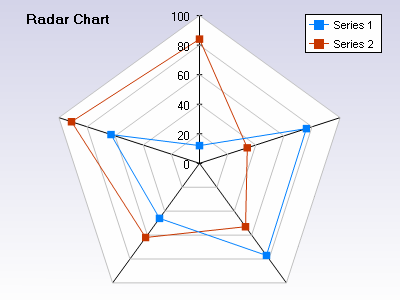
\includegraphics[width=0.5\linewidth]{images/radar}
	\caption{Dashboard Example - Radar Plot} 	
  	\label{fig:radar}
\end{figure}

The idea of a single visualisation method which allows to answer to any hypothesis is desirable, but not probable.  Unfortunately, the reliability of the methods depend on the system complexity and not only on the complexity of the method itself. Thus, this level of analysis may not be able to represent the entire system complexity. The Steady State condition represents another point of weakness. If it is not reached by all the variable involved, the analysis generalisation can not be granted and dashboard relevance becomes frail. Further levels of analysis are required, at least for a better comprehension of those unpredictable results that refute even naive hypothesis, formulated on well known theoretical truths.


\subsubsection{Level 1 -  Statistical Values Comparison}\label{sec:heaven-level1}

This Analysis level focuses on a single variable at time (Latency, Memory ecc.), in a certain statistical condition (Maximum, Minimum, Mean Value ecc.) exploiting \textit{Inter-Experiment} comparison. 

To verify an hypothesis researches design and execute multiple experiments which variates for few parameters. This analysis is focused on the entries experiment set. The experiments must be arranged into an smart layout that highlights the differences between experiments upon one or more well-defined characteristics. The analysis involves one variable at time, comparing the results over the experiment set. 

The aim of Level 1 is identifying which parameter, if any, determines behaviour of the solution w.r.t the observed variable. \name enables two possible analysis approaches within Level 1:
\begin{itemize}
\item \textit{Quantitative} -  The comparison results are present in percentage form, quantifying how much a solution is better than another one under some conditions. 
\item \textit{Qualitative} - it is a simplification of the Quantitative approach. Sometimes we only need to understand which solution is the best, without focusing on numeric values. The Qualitative approach requires the definition of a tolerance threshold, for example 5\%, to distinguish when a solution is better, worse or equal to another one.
\end{itemize}

\subsubsection{Level 2 - Patter Identification}\label{sec:heaven-level2}

The comparison of a single statistical value over multiple variable (Level 0) or a single one (Level 1) may be not sufficient to explicit the RSP Engine behaviour. Starting from Level 2, visual analysis for \textit{Inter-Experiment} comparison is introduced. As in Level 1 the investigation involves a single variable over the entire experiment set, disposed into an easy-to-ready layout which points out experiment differences. Level 2 instead enables the comparison of the experiment set, presenting result data in a graphical way, which shows the system behaviour over all the experiment execution.

The aim of this level is evidencing if a certain variable a some patterns among the experiment set. How to choose the correct graphical representation depends on the variable nature and requires specific analysis. However, the most common ones for time-series are time domain form, value distribution or frequency domain representations. In general Level 2 allows to visualise how the system behaves, which is not visible with a mere model investigation.

\subsubsection{Level 3 - Visual Comparison}\label{sec:heaven-level3}

The Level 3 is the bottom level of the investigation stack. It focuses on a single solution at time and it exploits both \textit{Inter-Experiment} comparison, with the aim to understand how different experiment execution are related or to  \textit{Intra-Experiment} comparison, with the goal of pointing out the relation between the variables over all the experiment. In the first case, Level 3 reproduces the Dashboard idea but over all the experiment execution. In the second case instead, it extends what done in Level 1 and 2, but focusing on a single visualisation at time.

\begin{figure}[htb]
  \centering
	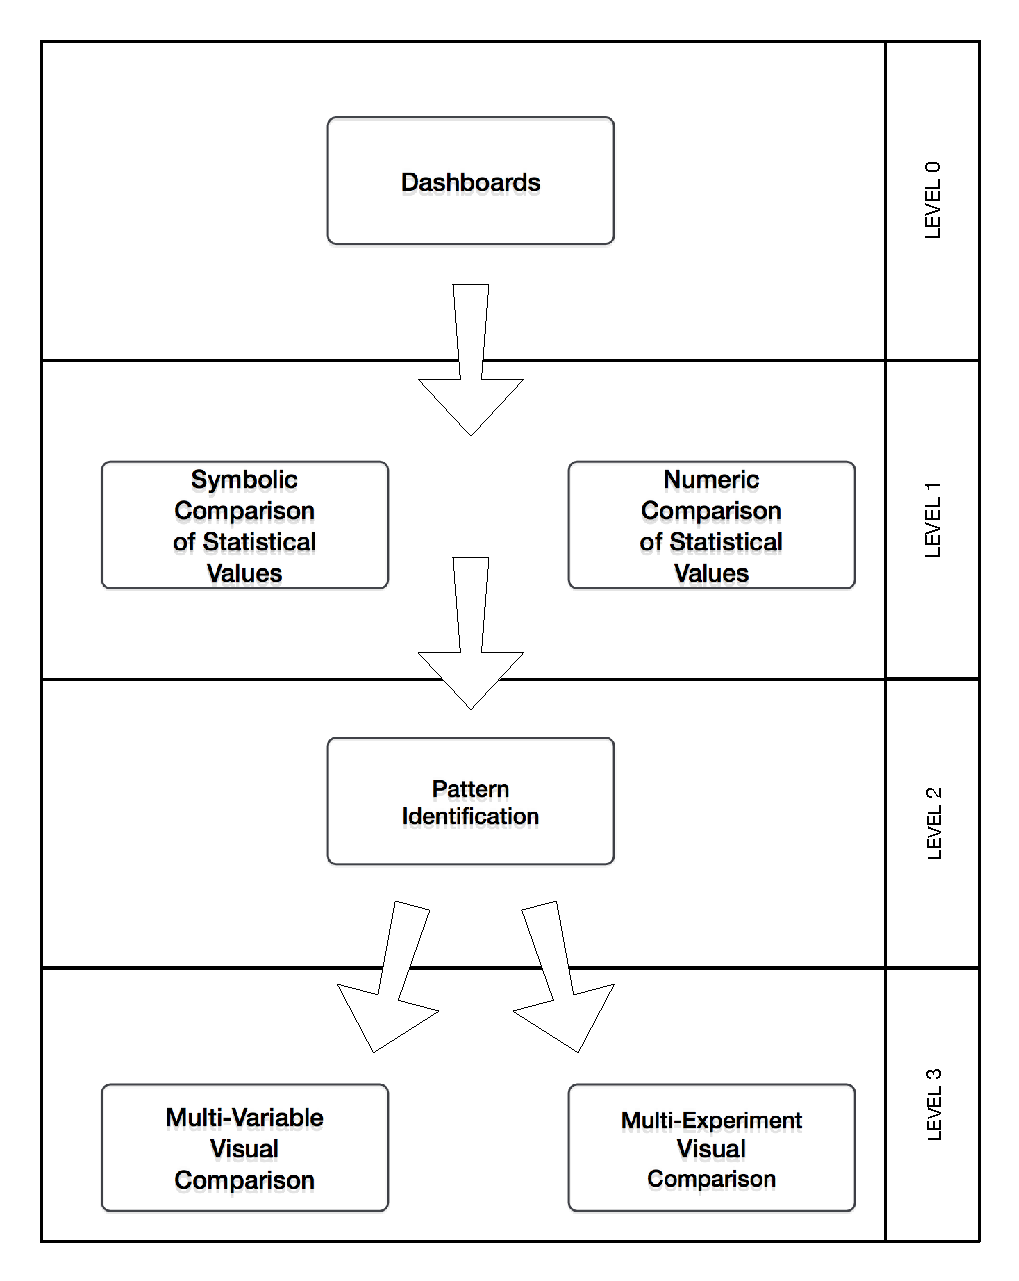
\includegraphics[width=\linewidth]{images/analysis-method}
	\caption{Analysis method stack. The level of analysis grows from the top to the bottom} 
  	\label{fig:analysis-method}
\end{figure}



